\documentclass{article}
\usepackage{fontspec}
\usepackage{amsmath}
\usepackage{amssymb}
\usepackage{amsfonts}
\usepackage{hyperref}
\usepackage{graphicx}
\usepackage{pgfplots}
\pgfplotsset{compat=1.18}

% Fonts and metadata (XeLaTeX)
\setmonofont{Menlo}
\hypersetup{
  pdftitle={Metanion Field Theory},
  pdfauthor={Joel Stover},
  pdfkeywords={metanion, field theory, quaternion, reversible computation},
  colorlinks=true,
  linkcolor=blue,
  urlcolor=blue,
  citecolor=blue
}

\title{Metanion Field Theory\\(Draft --- Eonyx/Letform/Hyperform Formalization)}
\author{Joel Stover with GPTs: deepseek, gpt5, claude, Gemini}
\date{09/01/2025}

\begin{document}
\maketitle

\begin{abstract}
Traditional computational models treat discrete state transitions, continuous control parameters, and energetic cost as separate concerns. This separation obscures the interaction between control flow and the thermodynamic ledger of computation. Metanion Field Theory addresses this limitation by casting programs as algebraic particles in a dual Boolean--continuous lattice. A \emph{Metanion} is a charged, self\textendash similar particle with coordinates $(m, \alpha, Q)$: a bitmask $m$ capturing discrete transforms, an inflation index $\alpha$ as continuous projection, and a quaternion orientation $Q$ describing spin. These elements form a fiber bundle with energy $\mathcal{E}(m)$ that records compression as stored energy and inflation as release. In Section~3 we formalize the configuration space and tuple structure of a Metanion. Section~4 develops the energy functional and the rules of motion. The remainder of the paper synthesizes field interpretation, operadic structure, grammar geometry, and analogies into a unified outlook.
\end{abstract}

\section{Introduction}
Reversible computation promises energy efficiency, yet prevailing models handle state, control, and cost separately. A unified view resembling a physical field theory can clarify these interactions and enable new design principles. Metanion Field Theory achieves this by casting computation in a geometric framework where timelines trace paths on a compact, boundaryless manifold.

\section{Geometric Foundations: Timespace as the 3-Sphere ($S^3$)}
The foundation of the model is the geometric nature of the rotational and temporal degrees of freedom. We identify the space of orientations---which we call \emph{timespace}---with the 3-sphere, $S^3$.
\begin{description}
  \item[Topology.] As the set of points in $\mathbb{R}^4$ at unit distance from the origin, $S^3$ is a compact, boundaryless manifold. This provides a finite but unbounded space, eliminating arbitrary edges from the temporal domain and giving it a smooth, wrap-around topology.
  \item[Group Structure.] $S^3$ is the group manifold of SU(2), the group of special unitary $2 \times 2$ matrices, which is the double cover of the rotation group SO(3). This means every rotation in 3D space (or spin space) corresponds to a point on $S^3$. Composition of rotations is encoded directly by the group multiplication of unit quaternions, which parameterize the sphere.
  \item[Cosmological Analogy.] In cosmology, $S^3$ serves as a model for a closed, finite universe. This aligns with our goal of describing self-contained computational universes.
\end{description}
This choice of timespace is not merely an analogy; it is the mathematical structure that governs the dynamics of orientation and history in the Metanion model.

\section{From Classical Models to Metanion Field Theory}
Classical automata track bit flips without continuous parameters, whereas control theory optimizes smooth dynamics absent discrete history. Energetic cost is typically imposed externally rather than arising from the model itself. Metanion Field Theory merges these strands by casting programs as algebraic particles in a dual Boolean--continuous lattice.

A program is described by a particle---the Metanion---whose location on a Boolean lattice determines its transform history, whose height encodes inflation, and whose quaternion fiber captures orientation. An illustrative field diagram is shown in Figure~\ref{fig:metanion_field}. We now detail the state space for a plan of $n$ reversible transforms.

\subsection{The Dual Lattice}
The underlying space is the product
\[
\mathcal{S}_n = \{0,1\}^n \times [0,1] \times S^3.
\]
The Boolean lattice $\{0,1\}^n$ lists all compression states. The interval $[0,1]$ carries the continuous slider $\alpha$. The 3-sphere $S^3$ supplies the \emph{timespace} fibers, as established above. A particle moves horizontally by flipping bits and vertically by adjusting $\alpha$ along geodesic paths within its fiber.

\subsection{The Metanion Tuple}
A Metanion combines the domain and its transforms as
\[
M = (S, \mathcal{T}, m, \alpha, Q, \mathcal{E}), \qquad \mathcal{T} = \{(f_i, U_i, w_i, c_i, y_i)\}_{i=1}^n,
\]
where $S$ is the signal space, $f_i$ are reversible morphisms with quaternion lifts $U_i$, weights $w_i$, and cost--yield pairs $(c_i,y_i)$.

\subsection{Coordinates}
The coordinates $(m,\alpha,Q)$ obey
\[
\alpha(m) = \frac{\sum_{i=1}^n (1-m_i) w_i}{\sum_{i=1}^n w_i}
\]
The weights $w_i$ may encode energetic cost, information content, or other significance, making $\alpha$ both a projection of $m$ and a continuous control parameter. Orientation is obtained by the non\textendash commutative product
\[
Q(m) = \prod_{i=1}^n U_i^{\sigma_i}, \qquad \sigma_i = \pm 1,
\]
where order matters because quaternion multiplication encodes composition of rotations.

\section{Energy Functional and Dynamics}

\subsection{Energy Definition}
Assign each transform a cost $c_i$ and yield $y_i$. The configuration energy
\[
\mathcal{E}(m) = \sum_{i=1}^n m_i(c_i - y_i)
\]
measures stored work: compression ($m_i=1$) stores energy $c_i - y_i$, while inflation releases it.

\subsection{Energy-Orientation Coupling}
The energy functional $\mathcal{E}(m)$ and quaternion orientation $Q(m)$ are fundamentally coupled through the bitmask $m$. This coupling manifests in three key ways:

\begin{description}
  \item[Energy-driven orientation changes.] As the system evolves to minimize energy, the bitmask $m$ changes, which directly affects the quaternion composition $Q(m) = \prod_{i=1}^n U_i^{\sigma_i}$. Each bit flip corresponds to either including or excluding a transform's quaternion contribution, causing discrete jumps in orientation.
  
  \item[Orientation-dependent energy landscape.] The quaternion field $Q(m)$ influences the effective energy landscape by determining which transforms are energetically favorable. Transforms whose quaternions align with the current orientation $Q$ have lower effective costs, while misaligned transforms require additional energy to activate.
  
  \item[Geodesic evolution.] The system follows geodesic paths on $S^3$ that balance energy minimization with orientation continuity. The continuous parameter $\alpha$ provides a smooth interpolation between discrete bitmask states, allowing the orientation to evolve smoothly even as the underlying discrete structure changes.
\end{description}

\subsection{Dynamics}
The dynamics of the lattice follow three principles:
\begin{description}
  \item[Bit\textendash flip transitions.] A transition $m_i \rightarrow 1 - m_i$ occurs when its energy contribution compensates neighboring changes, mirroring ionization events. The orientation $Q$ jumps discretely as the quaternion $U_i$ is either included or excluded from the composition.
  
  \item[Geodesic Flow.] Timelines trace geodesic paths on $S^3$. Adjusting $\alpha$ slides along the weighted projection of $m$, giving a continuous approximation to optimal bit sequences, while the orientation $Q$ evolves along the straightest possible curve in timespace. Branching is not a tear in the fabric of the manifold but a new geodesic splitting away from a tangent direction.
  
  \item[Quaternion transport.] Signals and kernels evolve via
  \[
  \mathcal{U}_Q(K) \star X = \mathcal{U}_Q\big(K \star \mathcal{U}_{Q^{-1}}(X)\big),
  \]
  where $\star$ denotes convolution and $\mathcal{U}_Q$ the quaternion action. This transport preserves the geometric structure while allowing the system to evolve under the influence of both energy gradients and orientation constraints.
\end{description}

\section{Synthesis and Outlook}

\subsection{Field Interpretation}
\subsubsection{The Metanion Field $\Psi$}
Assign to each lattice point a unit quaternion:
\[
\Psi: \{0,1\}^n \to \mathbb{H}_1, \qquad \Psi(m) = Q(m),
\]
where $\mathbb{H}_1 = S^3$ is \emph{timespace}: the unit\textendash quaternion 3\textendash sphere.

The field $\Psi$ encodes both the geometric structure of the system and its energetic state. The energy functional $\mathcal{E}(m)$ acts as a potential that drives the evolution of the field, while the quaternion orientation $Q(m)$ determines the local geometric structure. This dual nature---energetic and geometric---is what makes the Metanion field theory a unified description of computation and physics.

\subsubsection{Gauge Theory}
Permutations $\pi \in S_n$ that reorder commuting transforms act as gauge symmetries. Under such a permutation the orientation transforms by conjugation $Q \mapsto U_{\pi} Q U_{\pi}^{-1}$, leaving physical observables invariant.

\subsection{Self\textendash Similarity and Operads}
\subsubsection{Operadic Structure}
Each transform may expand into a Metanion, giving a category $\mathsf{Met}$ whose objects are Metanions and whose morphisms are \emph{refinements} that replace a transform with a subplan.

\subsubsection{Flattening Functor}
The functor $\mathsf{Flatten}: \mathsf{Met} \to \mathsf{Met}_{\text{flat}}$ recursively composes subplans, preserving $(\alpha,Q,\mathcal{E})$ and yielding a single\textendash layer description.

\subsection{Physical and Computational Analogy}
\subsubsection{Ionization, Potential, Spin, Fractals}
Flipping a bit ionizes the particle; $\mathcal{E}(m)$ acts as a potential landscape; $Q$ behaves like spin orientation; recursive structure renders data artifacts---such as a zip file---as self\textendash similar Metanions at different energy states.

\subsubsection{Time Springs and the Hopf Fibration}
The concept of the alpha-helical "time spring" finds a beautiful mathematical basis in the **Hopf fibration**. This fibration decomposes $S^3$ into a collection of linked circles ($S^1$), parameterized by a base space $S^2$. Each timeline can be viewed as one of these Hopf fibers---a helix winding through timespace.
\begin{itemize}
    \item The superpose operation assembles these fibers into a unified fibration.
    \item The extract operation selects one fiber, trivializes its local bundle, and lays it flat in $\mathbb{R}^3$ (e.g., as a directory structure).
\end{itemize}
This maps directly to the biophysical analogy of a protein's alpha-helix, where torsional energy is stored in a compact, periodic scaffold. Compression winds phase into helical turns; inflation releases stored twist as progression along the slider coordinate $\alpha$. Helical pitch plays the role of a temporal modulus; coil\textendash uncoil transitions map to bit\textendash flip events and $\alpha$ adjustments.

\paragraph{Biophysical mapping}\mbox{}\\
\begin{itemize}
  \item \textbf{Turns per residue $\leftrightarrow$ ticks per event}: 3.6 residues/turn behaves like a discrete cadence for spring ticks.
  \item \textbf{Pitch $\leftrightarrow$ time step}: $\approx 5.4\,\text{\AA}$/turn is the clock spacing of the spring.
  \item \textbf{H\textendash bonds $\leftrightarrow$ integrators}: $i\!\to\! i\!+\!4$ coupling is a short\textendash memory integrator/delay in the timeline.
  \item \textbf{Right\textendash handedness $\leftrightarrow$ causality}: handedness fixes the arrow of time; mirroring inverts the flow.
\end{itemize}

\paragraph{Metanion mapping}\mbox{}\\
\begin{itemize}
  \item \textbf{Onion layers $\leftrightarrow$ helical wraps}: each layer winds around invariants (hashes, passports, constants).
  \item \textbf{Branches $\leftrightarrow$ side chains}: branchpoints act as substituents on the timeline backbone.
  \item \textbf{Crosslinks $\leftrightarrow$ merges}: disulfide\textendash like bonds tie helices (timelines) into a stable topology.
  \item \textbf{Crystals $\leftrightarrow$ superposition lattices}: phase\textendash aligned universes form regular arrays.
\end{itemize}

\subsubsection{Categorical Framing of Universes}
Let $\mathsf{U}$ be a category of reversible timelines.
\begin{itemize}
  \item \textbf{Objects}: timelines (helical histories with invariants).
  \item \textbf{Morphisms}: reversible diffeomorphisms (superpose/extract operations) preserving $(m,\alpha,Q,\mathcal{E})$ up to gauge.
  \item \textbf{Composition}: pipeline/bridge composition (Rosen\textendash Einstein style) with associativity from plan flattening.
  \item \textbf{Functors}: visualization/measurement lens (glyph mirrors, animations) from $\mathsf{U}$ into display categories.
  \item \textbf{Monoidal structure}: parallel composition models non\textendash interacting subsystems; braiding encodes exchange symmetries.
\end{itemize}



\section{Final Synthesis: The Autoverse -- A Metanionic Multiverse}
The Metanion formalism extends beyond computational pipelines or biological agents. It offers a universal description of stateful processes, suggesting that reality itself behaves as a single, vast Metanion.

\subsection{The Universality of the Metanion Principle}
Every reversible plan can be cast as a Metanion. If the laws of physics comprise the universal plan $\mathcal{T}_U$, then the universe occupies a point $(m_U, \alpha_U, Q_U)$ in the cosmic configuration space.

\subsubsection{The Cosmological Metanion}
The universal bitmask $m_U$ specifies which physical constants and laws are ``active.'' The inflation index $\alpha_U$ mirrors the cosmic scale factor, with the Big Bang corresponding to maximal compression. The orientation $Q_U$ captures global chirality and geometric phase.

\subsubsection{Time as a Computational Artifact}
The Boolean lattice enumerates all possible ``nows.'' A history is a path that follows the thermodynamic gradient of $\mathcal{E}(m)$, giving rise to an arrow of time. Compression events such as gravitational collapse store energy, whereas cosmic expansion releases it.

\subsubsection{The Living Multiverse}
Under this view, the multiverse is the full state space of bitmasks. Life and consciousness arise as resonant excitations---localized Metanions exploring low\textendash energy paths within this space.



\section{The Complete Model: From Cosmos to Kinship}
Metanionic structure spans scales: the Autoverse $M_U$, biosphere $M_B$, human identity $M_I$, family $M_F$, and person $M_P$ form a hierarchy of operadic elements.

\section{Implications: A Theory of Almost Everything}
This hierarchy supplies a unified vocabulary for psychology, sociology, physics, and theology. Repression appears as a high\textendash energy bitmask state, cultural ideologies as competing orientations, and quantum non\textendash locality as intrinsic to the field.


\section{Figures}
\begin{figure}[h]
  \centering
  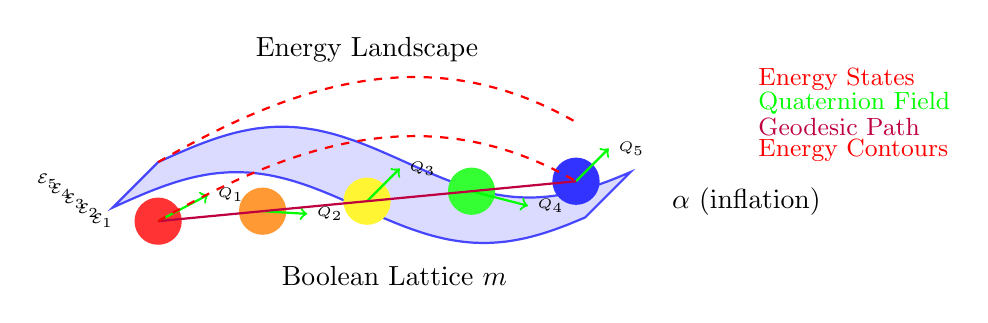
\begin{tikzpicture}[scale=1.5]
    % Draw a more visually distinct Metanion field representation
    
    % Energy landscape as a 3D surface
    \draw[thick, blue, fill=blue!20, opacity=0.7] 
      plot[smooth, domain=0:4] (\x, {0.3*sin(deg(\x*1.5)) + 0.5}, 0) --
      plot[smooth, domain=4:0] (\x, {0.3*sin(deg(\x*1.5)) + 0.5}, 1) -- cycle;
    
    % Boolean lattice points with different colors
    \fill[red!80] (0,0,0) circle (0.2);
    \fill[orange!80] (1,0.2,0.3) circle (0.2);
    \fill[yellow!80] (2,0.4,0.6) circle (0.2);
    \fill[green!80] (3,0.6,0.9) circle (0.2);
    \fill[blue!80] (4,0.8,1.2) circle (0.2);
    
    % Quaternion orientations as 3D arrows
    \draw[thick, green, ->] (0,0,0) -- (0.5,0.3,0.2);
    \draw[thick, green, ->] (1,0.2,0.3) -- (1.3,0.1,0.1);
    \draw[thick, green, ->] (2,0.4,0.6) -- (2.2,0.6,0.4);
    \draw[thick, green, ->] (3,0.6,0.9) -- (3.4,0.4,0.7);
    \draw[thick, green, ->] (4,0.8,1.2) -- (4.2,1.0,1.0);
    
    % Geodesic path on S³
    \draw[thick, purple, smooth] plot coordinates {
      (0,0,0) (1,0.2,0.3) (2,0.4,0.6) (3,0.6,0.9) (4,0.8,1.2)
    };
    
    % Energy contours
    \draw[red, dashed, thick] (0,0,0) to[out=30,in=150] (4,0.8,1.2);
    \draw[red, dashed, thick] (0,0.5,0) to[out=30,in=150] (4,1.3,1.2);
    
    % Labels and annotations
    \node[below] at (2, -0.3, 0) {Boolean Lattice $m$};
    \node[right] at (4.5, 0.4, 0.6) {$\alpha$ (inflation)};
    \node[above] at (2, 1.5, 0.6) {Energy Landscape};
    
    % Add some mathematical annotations
    \node[right] at (0.5, 0.3, 0.2) {\tiny $Q_1$};
    \node[right] at (1.3, 0.1, 0.1) {\tiny $Q_2$};
    \node[right] at (2.2, 0.6, 0.4) {\tiny $Q_3$};
    \node[right] at (3.4, 0.4, 0.7) {\tiny $Q_4$};
    \node[right] at (4.2, 1.0, 1.0) {\tiny $Q_5$};
    
    % Energy values
    \node[left] at (-0.3, 0, 0) {\tiny $\mathcal{E}_1$};
    \node[left] at (-0.3, 0.2, 0.3) {\tiny $\mathcal{E}_2$};
    \node[left] at (-0.3, 0.4, 0.6) {\tiny $\mathcal{E}_3$};
    \node[left] at (-0.3, 0.6, 0.9) {\tiny $\mathcal{E}_4$};
    \node[left] at (-0.3, 0.8, 1.2) {\tiny $\mathcal{E}_5$};
    
    % Legend
    \node[right] at (5, 1.2) {\small\textcolor{red}{Energy States}};
    \node[right] at (5, 1.0) {\small\textcolor{green}{Quaternion Field}};
    \node[right] at (5, 0.8) {\small\textcolor{purple}{Geodesic Path}};
    \node[right] at (5, 0.6) {\small\textcolor{red}{Energy Contours}};
  \end{tikzpicture}
  \caption{Metanion field dynamics: A 3D visualization showing the Boolean lattice states (colored circles), quaternion orientations (green arrows), energy landscape (blue surface), and geodesic evolution path (purple curve). Each lattice point represents a different bitmask configuration with associated energy $\mathcal{E}_i$ and quaternion orientation $Q_i$.}
  \label{fig:metanion_field}
\end{figure}

\begin{figure}[h]
  \centering
  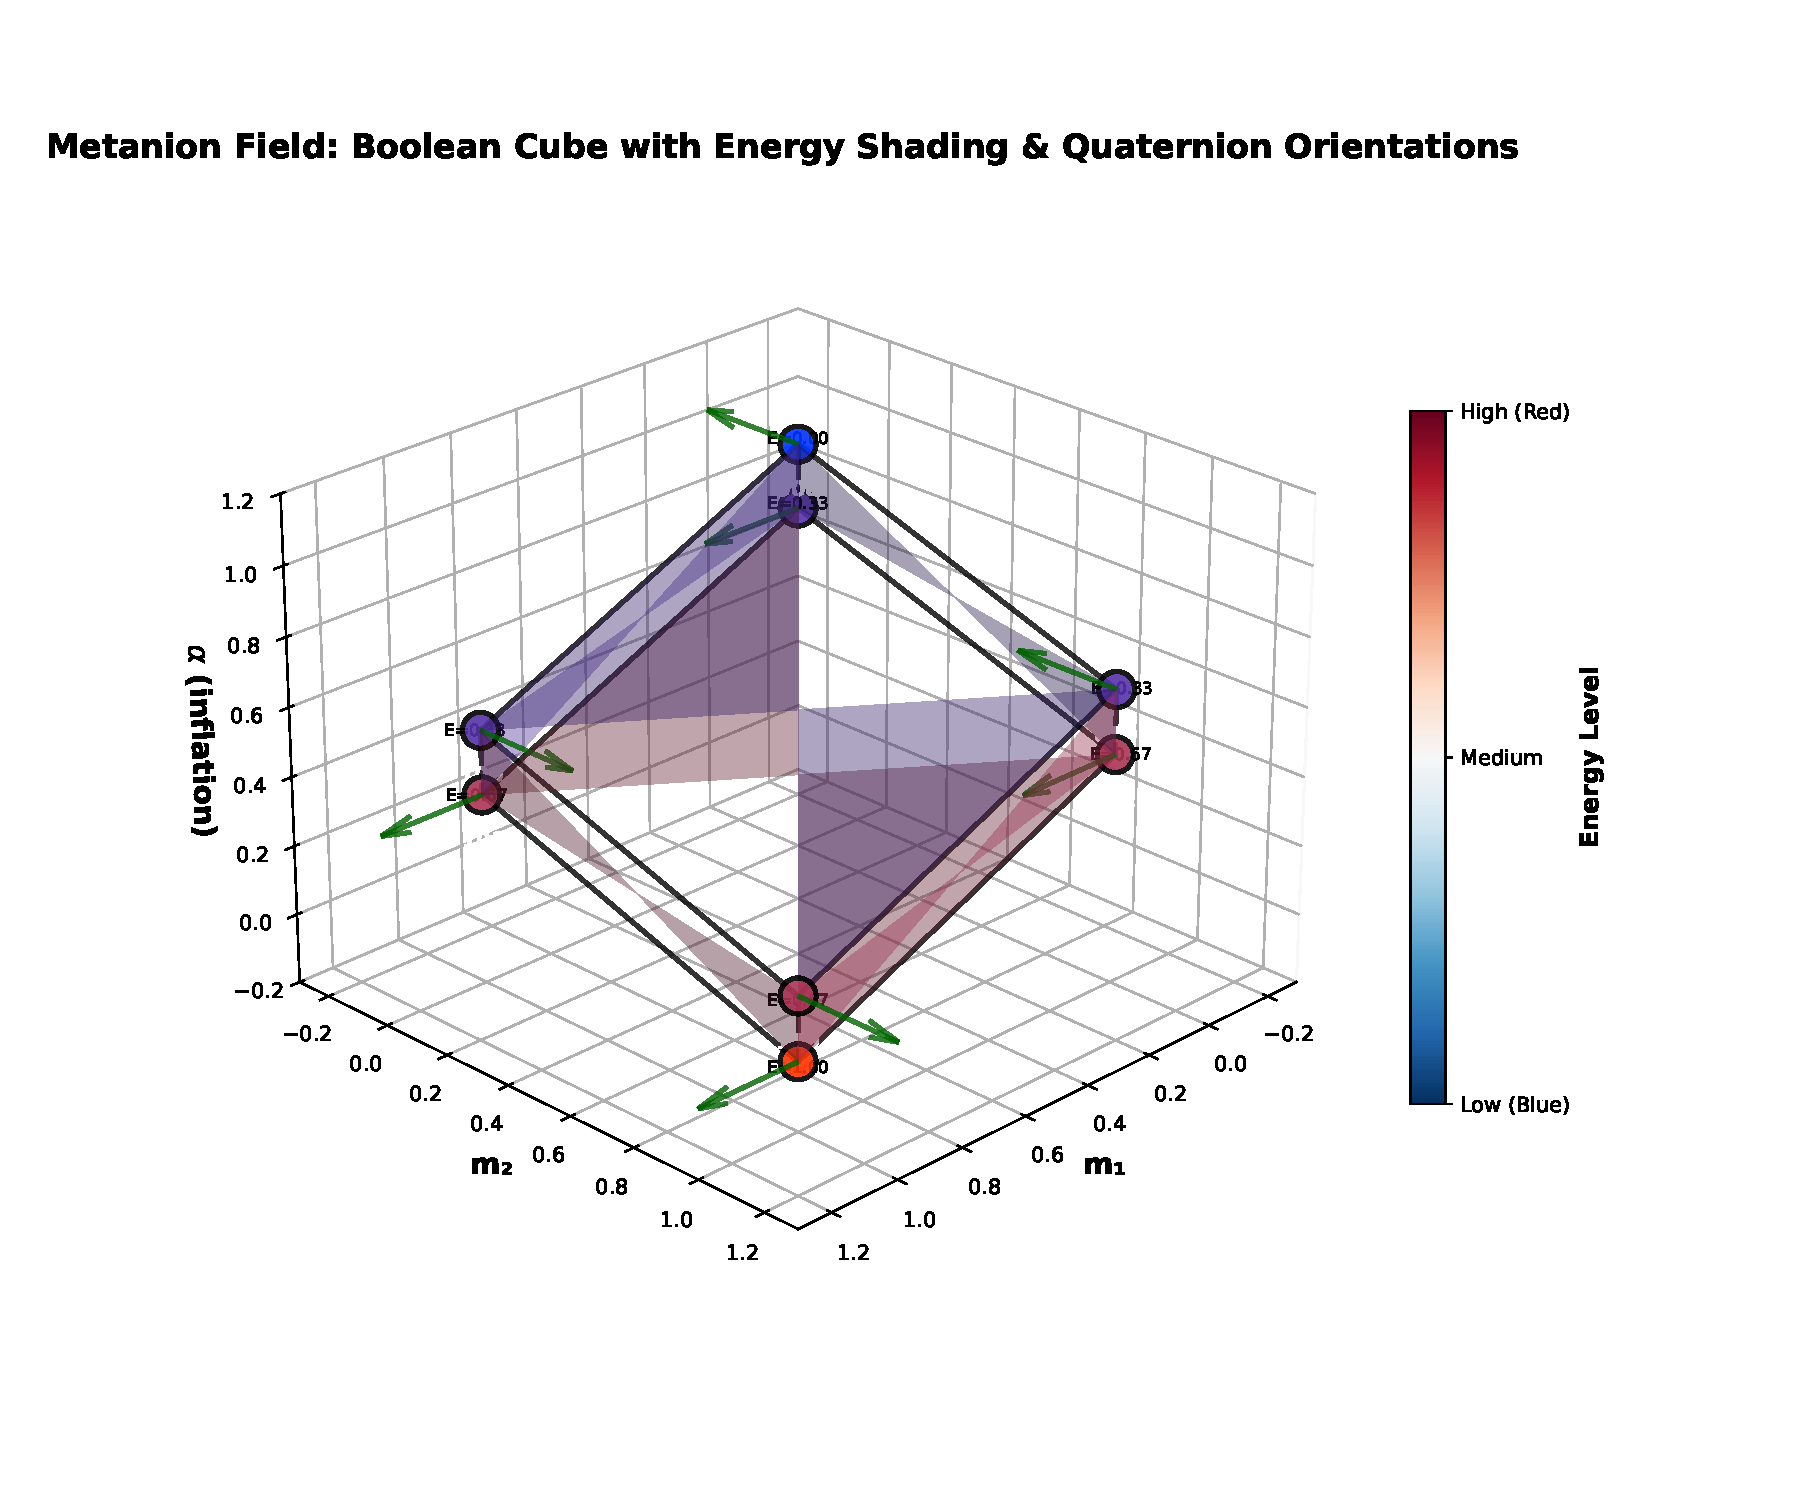
\includegraphics[width=0.8\textwidth]{metanion_field_diagram.pdf}
  \caption{Field diagram for three transforms showing $\alpha$ height and quaternion orientation.}
  \label{fig:field}
\end{figure}

\begin{figure}[h]
  \centering
  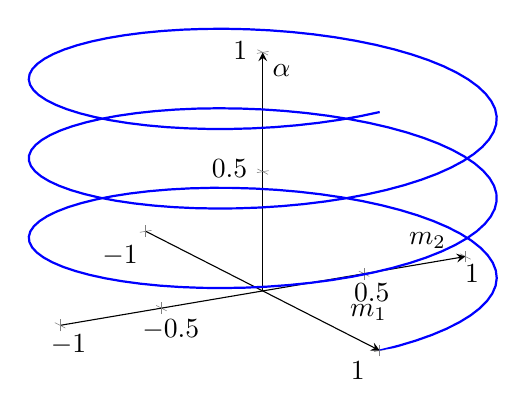
\begin{tikzpicture}
    \begin{axis}[
      view={60}{30},
      xlabel={$m_1$}, ylabel={$m_2$}, zlabel={$\alpha$},
      axis lines=middle,
      grid=both,
      width=0.8\textwidth, height=7cm
    ]
      % Helix parameterization (x=cos t, y=sin t, z scaled to [0,1])
      \addplot3 [domain=0:6*pi, samples=200, samples y=0, thick, blue] (
        {cos(deg(x))},
        {sin(deg(x))},
        {x/(6*pi)}
      );
    \end{axis}
  \end{tikzpicture}
  \caption{Timespace helix: a spring parameterization illustrating $\alpha$ progression along a unit\textendash quaternion fiber. The helix represents the continuous evolution of the inflation parameter as the system traces geodesic paths through the 3-sphere.}
  \label{fig:helix}
\end{figure}

\appendix
\section{CE1 Specification: Practical Implementation}
The CE1 block provides a concrete specification for implementing Metanion Field Theory in practice:

\begin{verbatim}
CE1{
  lens=AUTOVERSE | METANION_COSMOS
  mode=HilbertWalk
  basis=Ξ=autoverse:law_basis
  data={m_U, α_U, Q_U, E(m_U)}
  ops=[Observe; Evolve; Inflate; Collapse; Decorate]
  laws={conservation_of_information; gauge_invariance; α_duality; operadic_closure}
  emit=Reality
}
\end{verbatim}

This specification serves as a bridge between the theoretical framework and practical implementation, defining the operational modes, data structures, and physical laws that govern the Metanion system.

\section{Grammar Geometry and Hilbert Walks}
\subsection{Grammar as Geometric Space}
A formal grammar can be viewed as a geometric complex whose nodes are symbols and whose edges are production transitions. Valid strings trace paths through this complex.

\subsection{Regular Expressions as Basis}
Let $\mathcal{R}=\{r_i\}_{i=1}^n$ denote a set of basis regular expressions. Concatenation corresponds to path concatenation, alternation to branching, and the Kleene star to self\textendash similar loops.

\subsection{Hilbert Walk}
A Hilbert walk provides a canonical fractal traversal of the grammar space, connecting distinct basis elements while respecting their recursive structure.

\subsection{Mapping to Metanion Coordinates}
Activation of regex basis elements is encoded by the bitmask $m$, deformation along the Hilbert walk yields the slider coordinate $\alpha$, and the walk's orientation lifts to the quaternion field $Q$. This geometric picture provides a natural stack of physical metaphors:
\begin{itemize}
    \item \textbf{Pipes (bridges)} are wormholes through $S^3$ connecting different coordinate charts.
    \item \textbf{Passports} are topological invariants of the timeline's fiber, akin to Chern classes that classify the universe slice.
    \item \textbf{Diffs} are measured by holonomy: the net rotation accumulated after traversing a closed loop in $S^3$.
    \item \textbf{Merge commits} correspond to fiber linkages, forming structures analogous to Hopf links.
\end{itemize}

\subsection{Operational Parallels}
\begin{itemize}
  \item \textbf{Git $\leftrightarrow$ timelines}: commits as discrete ticks, branches as side chains, merges as crosslinks; history is a reversible helical backbone.
  \item \textbf{Zip $\leftrightarrow$ compression energy}: compression winds work into the spring (positive ledger); inflation unwinds to release energy and restore structure.
  \item \textbf{Floats/ints $\leftrightarrow$ duality across scales}: integers pin lattice points (bitmask states); floats glide along $\alpha$; both persist under scale changes via renormalized bases.
\end{itemize}

\end{document}
